% main_kr.tex
\documentclass[11pt,a4paper]{article}

% ---- Language / Font ----
\usepackage[T1]{fontenc}
\usepackage[utf8]{inputenc}
\usepackage{kotex}

% ---- Layout ----
\usepackage[margin=1in]{geometry}
\usepackage{graphicx}
\graphicspath{{../../figures/}}

% ---- Math / Tables ----
\usepackage{amsmath,amssymb}
\usepackage{booktabs}
\usepackage{array}
\usepackage{longtable}

% ---- Lists / Links ----
\usepackage{enumitem}
\usepackage[hidelinks]{hyperref}

% ---- Bibliography ----
\usepackage[numbers]{natbib}

\title{라우팅 공격 하에서 복원력을 갖춘 Trust-Aware Backpressure RPL}
\author{이건형}
\date{}

\begin{document}
\maketitle

\begin{abstract}
Low-Power and Lossy Networks(LLNs)는 lossy wireless link와 congestion 환경에서도 안정적인 라우팅을 위해 RPL과 backpressure 기반 변형인 BRPL에 의존한다. 그러나 기존 RPL/BRPL은 data-plane forwarding을 조작하거나 control-plane advertisement(예: rank)를 조작하는 insider routing attack을 명시적으로 고려하지 않으며, 토폴로지와 라우팅 구조에 따라 특정 attack intensity를 넘어서면 성능이 급격히 붕괴(collapse)할 수 있다. 본 논문은 BRPL의 라우팅 결정에 trust-derived penalty를 경량으로 통합한 \emph{Trust-Aware BRPL}을 제안한다. Data-plane reliability는 EWMA smoothing을 적용한 Beta-based estimator로 모델링하고, control-plane anomaly는 rank inconsistency 및 stability signal을 사용해 포착한다. Contiki-NG/Cooja 환경에서 attack intensity, topology class, network scale에 대한 재현 가능한 parameter sweep을 수행하며, BRPL과 Trust-Aware BRPL을 packet delivery ratio(PDR), end-to-end delay, control overhead, parent churn 측면에서 비교한다. 실험 결과(추후 삽입)는 trust parameter가 collapse threshold를 어떻게 이동시키는지 정량화하고, 그에 따른 resilience--overhead trade-off를 분석하도록 구성된다.
\end{abstract}

\noindent\textbf{Keywords:} RPL, BRPL, Backpressure, Trust, LLN, IoT Security, Selective Forwarding, Sinkhole, Contiki-NG, Cooja

\section{Introduction}
\label{sec:intro}
LLNs는 엄격한 power/memory constraint 하에서 동작하는 IoT sensing 및 control 시스템에 널리 사용되며, lossy wireless link를 통해 통신한다. RPL은 DODAG formation, rank, parent selection에 기반한 LLN용 표준 IPv6 routing framework를 제공한다 \citep{rfc6550}. BRPL은 backpressure-inspired decision을 통해 RPL을 확장하여, congestion 상황에서 path diversity를 활용함으로써 throughput과 latency를 개선한다 \citep{moeller2016brpl}.

이러한 발전에도 불구하고, LLN 라우팅은 여전히 insider attack에 취약하다. 대표적인 위협으로는 (i) \emph{selective forwarding}(grayhole/blackhole) 공격이 있으며, compromised forwarder가 확률적으로 패킷을 drop한다. (ii) \emph{sinkhole} 공격은 misleading control-plane advertisement(예: rank manipulation)로 트래픽을 유인한 뒤 전달을 방해한다 \citep{karlof2003secure,wood2002dos,le2013rank,mayzaud2016taxonomy}. 경험적으로 이러한 공격은 \emph{phase-transition-like} 거동을 보인다: attack intensity가 낮을 때는 성능 저하가 제한적이지만, topology 및 routing structure에 의존하는 threshold를 넘어서면 성능이 급격히 붕괴한다.

\subsection{Goal and Approach}
\label{subsec:goal}
본 연구의 목표는 경량 trust signal을 BRPL decision process에 통합하여 이러한 collapse를 지연시키거나 완화하는 것이다. Heavy cryptographic mechanism이나 standalone intrusion detection을 도입하는 대신, trust를 routing metric의 \emph{penalty}로 통합한다. 이를 통해 의심 노드는 forwarder/parent로서 덜 선호되면서도, BRPL의 congestion-aware 이점을 유지하도록 유도한다.

\subsection{Contributions}
\label{subsec:contrib}
\begin{itemize}[leftmargin=*]
  \item \textbf{Trust-Aware BRPL design:} backpressure 기반 adaptivity를 유지하면서 untrustworthy neighbor를 down-weight하는 경량 trust-penalized BRPL metric을 제안한다.
  \item \textbf{Dual-plane trust modeling:} data-plane trust는 Beta estimation + EWMA smoothing으로, control-plane trust는 RPL semantics에서 도출한 rank inconsistency 및 stability signal로 모델링한다.
  \item \textbf{Reproducible evaluation framework:} Contiki-NG/Cooja 구현 및 scripted sweep을 통해 topology class, scale(S/M/L), attack intensity를 체계적으로 스윕하며 selective forwarding, sinkhole, combined attack을 평가한다.
  \item \textbf{Collapse-threshold analysis:} trust parameter가 collapse point를 어떻게 이동시키는지, 그리고 resilience가 overhead 및 churn과 어떻게 trade-off되는지 정량화하도록 결과를 구성한다.
\end{itemize}

\subsection{Paper Organization}
Section~\ref{sec:background}에서는 background 및 related work를 다룬다.
Section~\ref{sec:model}에서는 system/threat model을 정의한다.
Section~\ref{sec:design}에서는 Trust-Aware BRPL 설계를 제시한다.
Section~\ref{sec:impl}에서는 구현을 설명한다.
Section~\ref{sec:setup}에서는 실험 설정을 기술한다.
Section~\ref{sec:results} 및 Section~\ref{sec:discussion}에서는 결과 보고 및 논의를 수행한다.
Section~\ref{sec:conclusion}에서 결론을 맺는다.

\section{Background and Related Work}
\label{sec:background}
\subsection{RPL and BRPL}
RPL은 sink를 root로 하는 DODAG를 구성하고, rank를 통해 loop avoidance 및 convergence를 보장한다 \citep{rfc6550}. BRPL은 backpressure principle을 RPL에 접목하여 queue differential과 routing cost를 결합함으로써 congestion 하에서 throughput과 delay를 개선하고, 가능한 경우 multi-path를 활용한다 \citep{moeller2016brpl}.

\subsection{Routing Attacks in LLNs}
Selective forwarding 및 sinkhole/rank attack은 LLN에서 delivery와 stability를 심각하게 저하시킬 수 있는 대표적 위협으로 알려져 있다 \citep{karlof2003secure,wood2002dos,le2013rank,mayzaud2016taxonomy}. 특히 sinkhole은 misleading control-plane information으로 트래픽을 유인하며, critical path에 위치한 이후 disruption을 증폭시키기 쉽다.

\subsection{Trust-Based Routing}
Trust-based routing은 behavioral reliability를 routing decision에 반영하는 접근으로, direct observation 및/또는 reputation system을 활용한다 \citep{ganeriwal2004reputation,ganeriwal2008tosn,momani2010survey}. LLN에서는 wireless observation의 불완전성과 overhearing의 한계로 인해, full watchdog보다는 lightweight estimator와 smoothing 기법이 실용적이다.

\section{System and Threat Model}
\label{sec:model}
\subsection{System Model}
Contiki-NG 및 Cooja를 사용하여 RPL/BRPL routing을 포함하는 6LoWPAN/IPv6 LLN stack을 시뮬레이션한다. 트래픽은 sensor node에서 root로의 many-to-one periodic pattern을 따른다. 각 노드는 neighbor table을 유지하며 underlying routing logic에 따라 preferred parent를 선택한다 \citep{rfc6550,moeller2016brpl}.

\subsection{Threat Model}
단일 insider attacker를 고려한다(multiple attacker는 future work). 공격자는 정상 노드로 참여하되 다음 중 하나를 수행한다:
\begin{itemize}[leftmargin=*]
  \item \textbf{Selective forwarding:} forwarded traffic에 대해 확률적으로 packet drop을 수행하며, drop probability를 attack intensity로 스윕한다.
  \item \textbf{Sinkhole (rank manipulation):} control-plane 조작(예: artificially low rank advertisement)으로 트래픽을 유인하며, dropping과 결합되지 않는 경우에는 정상 forwarding을 수행한다.
  \item \textbf{Combined attack:} sinkhole attraction 이후 captured flow에 selective forwarding을 결합한다.
\end{itemize}
Root는 non-malicious하다고 가정한다. Cryptographic authentication 및 secure bootstrapping은 본 논문의 범위 밖이다.

\section{Trust-Aware BRPL Design}
\label{sec:design}
본 절에서는 trust signal을 정의하고, 이것이 BRPL decision을 어떻게 조절(modulate)하는지 기술한다. 관측 노드를 $i$, neighbor candidate(잠재적 parent/forwarder)를 $j$로 표기한다. Trust value는 $[0,1]$로 정규화되며 값이 클수록 신뢰도가 높다.

\subsection{Data-Plane Trust for Selective Forwarding}
\label{subsec:grayhole}
Forwarding reliability를 neighbor가 패킷을 성공적으로 전달할 확률로 모델링한다. $s_j$와 $f_j$는 각각 $j$에 귀속된 forwarding success/failure 이벤트의 관측치로 둔다(예: log-based inference). Bernoulli forwarding outcome에 대해 Beta prior $(\alpha_0,\beta_0)$를 적용하면 \citep{ganeriwal2004reputation,ganeriwal2008tosn}, posterior mean은
\begin{equation}
\hat{T}_{\text{gray}}(j)=\frac{\alpha_0+s_j}{\alpha_0+\beta_0+s_j+f_j}
\end{equation}
이다. Short-term noise를 줄이기 위해 EWMA smoothing을 적용한다:
\begin{equation}
T_{\text{gray}}(j;t)=\rho\,T_{\text{gray}}(j;t\!-\!1)+(1-\rho)\,\hat{T}_{\text{gray}}(j),
\end{equation}
여기서 $\rho\in[0,1)$는 smoothing 강도를 제어한다.

\subsection{Control-Plane Trust for Sinkhole Behavior}
\label{subsec:sinkhole}
Sinkhole attack은 주로 control-plane advertisement에 영향을 준다. RPL rank semantics는 feasible parent relation에 monotonicity constraint를 부과한다 \citep{rfc6550}. $R_i$를 노드 $i$의 current rank, $R_j$를 neighbor $j$가 광고(advertise)한 rank로 둔다. 다음을 정의한다:
\begin{equation}
\Delta_{ij}=R_j+\mathrm{MIN\_HOPRANKINC}-R_i.
\end{equation}
$j$가 $i$ 대비 implausibly low rank를 광고하면 $\Delta_{ij}$가 음수가 된다. Tolerance $\tau\ge 0$를 두고 deviation score를
\begin{equation}
s_{ij}=\max(0,\,-\Delta_{ij}-\tau)
\end{equation}
로 정의하며, 이를 exponential trust decay로 매핑한다 \citep{sun2005trust,chen2010trust}:
\begin{equation}
T_{\text{adv}}(j)=\exp(-\lambda_{\text{adv}}\,s_{ij}),
\end{equation}
여기서 $\lambda_{\text{adv}}>0$는 sensitivity를 설정한다.

Sinkhole behavior는 rank evolution 및 parent selection의 instability를 유발할 수 있다. Window $W$에 대해 rank increase를
\begin{equation}
\Delta R_i=R_i(t)-R_i(t-W)
\end{equation}
로 정의하고, $\kappa\ge 0$를 넘는 abnormal increase를 패널티한다:
\begin{equation}
u_i=\max(0,\,\Delta R_i-\kappa), \qquad
T_{\text{stab}}(t)=\exp(-\lambda_{\text{stab}}\,u_i).
\end{equation}
Control-plane signal은 곱셈적으로 결합한다:
\begin{equation}
T_{\text{sink}}(j)=\left(T_{\text{adv}}(j)\right)^{w_1}\left(T_{\text{stab}}(t)\right)^{w_2},
\end{equation}
여기서 $w_1,w_2\ge 0$는 각 신호의 weight이다.

\subsection{Total Trust Aggregation}
\label{subsec:totaltrust}
Data-plane trust와 control-plane trust는 weighted geometric mean으로 집계한다:
\begin{equation}
T_{\text{total}}(j)=\left(T_{\text{gray}}(j)\right)^{\alpha}\left(T_{\text{sink}}(j)\right)^{1-\alpha},
\end{equation}
여기서 $\alpha\in[0,1]$는 selective forwarding vs. sinkhole signal의 강조 비율을 제어한다.

\subsection{Trust-Penalized BRPL Metric}
\label{subsec:metric}
$BP_{ij}$를 노드 $i$에서 neighbor $j$에 대한 baseline BRPL weight/utility로 둔다(BRPL의 backpressure + cost 결합으로 정의됨) \citep{moeller2016brpl}. Trust penalty factor를
\begin{equation}
\phi(T)=\frac{T^{\gamma}}{1+\lambda\,(1-T)^{\gamma}},
\label{eq:phi}
\end{equation}
로 정의하며, $\lambda\ge 0$는 avoidance aggressiveness를, $\gamma\ge 1$은 risk sensitivity를 제어한다. Trust-aware metric은
\begin{equation}
BP^{\text{(trust)}}_{ij}=BP_{ij}\cdot \phi\!\left(T_{\text{total}}(j)\right)
\end{equation}
이다. 본 형태는 trust가 uniform할 때 ordering을 보존하면서, $\lambda$ 또는 $\gamma$가 증가할수록 low-trust neighbor를 강하게 down-weight한다. Tunable penalty parameter의 사용은 stochastic network optimization에서의 drift-plus-penalty 및 risk-sensitive control 직관과 부합한다 \citep{neely2010}.

\subsection{Algorithm Outline}
\label{subsec:algo}
각 decision epoch에서 노드 $i$는 다음을 수행한다:
\begin{enumerate}[leftmargin=*]
  \item Trust value(data-plane 및/또는 control-plane)를 업데이트하고 $[0,1]$로 clamp한다.
  \item 각 neighbor candidate $j$에 대해 $BP^{\text{(trust)}}_{ij}$를 계산한다.
  \item Trust-penalized objective를 최대화하는 preferred parent / forwarding next hop을 선택하며, churn 감소를 위해 optional hysteresis를 적용할 수 있다.
\end{enumerate}

\subsection{Overhead}
\label{subsec:overhead}
Trust 유지에는 노드당 $O(\deg)$ 값 저장이 필요하며, 여기서 $\deg$는 neighbor degree이다. Metric 계산은 decision당 $O(\deg)$ 산술 연산을 추가한다. 설계상 additional control packet은 요구되지 않으며, 추가 overhead는 변경된 routing dynamic(예: parent switching)에서 발생할 수 있다.

\section{Implementation in Contiki-NG}
\label{sec:impl}
Contiki-NG에서 Trust-Aware BRPL을 구현하기 위해 trust penalty를 BRPL metric computation 및 parent selection path에 통합하였다. Attacker node는
(i) selective forwarding을 위한 probabilistic forwarding drop,
(ii) sinkhole behavior를 위한 rank advertisement manipulation,
(iii) combined operation을 지원한다.

Routing decision에 사용되는 모든 trust 값은 simulation runtime 동안 각 노드에서 \emph{online}으로 계산되어 즉시 적용된다. 별도로 수행되는 trust engine의 \emph{offline} log-based analysis는 measurement/visualization/reproducibility 목적에 한정되며, offline 결과가 routing decision에 피드백되는 일은 없다.

재현성을 위해 seed/topology/attack parameter에 대한 batch experiment를 수행하고, Cooja log에서 metric을 추출하는 scripted pipeline을 유지한다. 구현 세부 파일명 및 스크립트는 본문에서는 생략하며, code repository와 함께 artifact로 제공할 수 있다.

\begin{figure}[t]
  \centering
  \includegraphics[width=0.9\linewidth]{architecture.pdf}
  \caption{Software architecture of Trust-Aware BRPL and its integration into the Contiki-NG protocol stack.}
  \label{fig:arch}
\end{figure}

\begin{figure}[t]
  \centering
  \includegraphics[width=0.9\linewidth]{trust_update_flow.pdf}
  \caption{Online trust update and routing decision flow executed at each node during simulation runtime.}
  \label{fig:trust-flow}
\end{figure}

\section{Experimental Setup}
\label{sec:setup}
\subsection{Simulation Environment}
Cooja의 UDGM Distance Loss radio model을 사용한다 \citep{osterlind2006cooja}. 별도로 명시하지 않는 한 simulation은 600\,s 동안 실행되며 warm-up은 120\,s로 둔다. Sensor node는 30\,s마다 root로 periodic traffic을 생성한다. RPL Trickle parameter는 stability와 control overhead 간 trade-off를 고려한 표준 구성을 따른다 \citep{rfc6550}.

\subsection{Topologies and Scales}
서로 다른 path diversity regime을 포괄하기 위해 다음 topology \emph{class}를 평가한다:
\begin{itemize}[leftmargin=*]
  \item \textbf{Grid:} high path diversity; attack이 부분적으로 bypass될 수 있음.
  \item \textbf{Two-cluster with bottleneck:} constrained cut; attacker가 bottleneck 근처에 위치할 때 attack effect가 증폭됨.
  \item \textbf{Corridor/chain:} low path diversity; 낮은 intensity에서 collapse가 발생할 수 있음.
  \item \textbf{Ring/spokes:} intermediate diversity; root-near 및 mid-path 영향이 두드러짐.
\end{itemize}
Network size는 S/M/L(예: root 포함 16/36/64 nodes)로 확장하되, class별 placement rule은 유지한다. Attacker placement는 ad-hoc tuning을 피하기 위해 rule-based selection(예: central relay candidate 또는 bottleneck vicinity)을 따른다.

\begin{figure}[p]
  \centering
  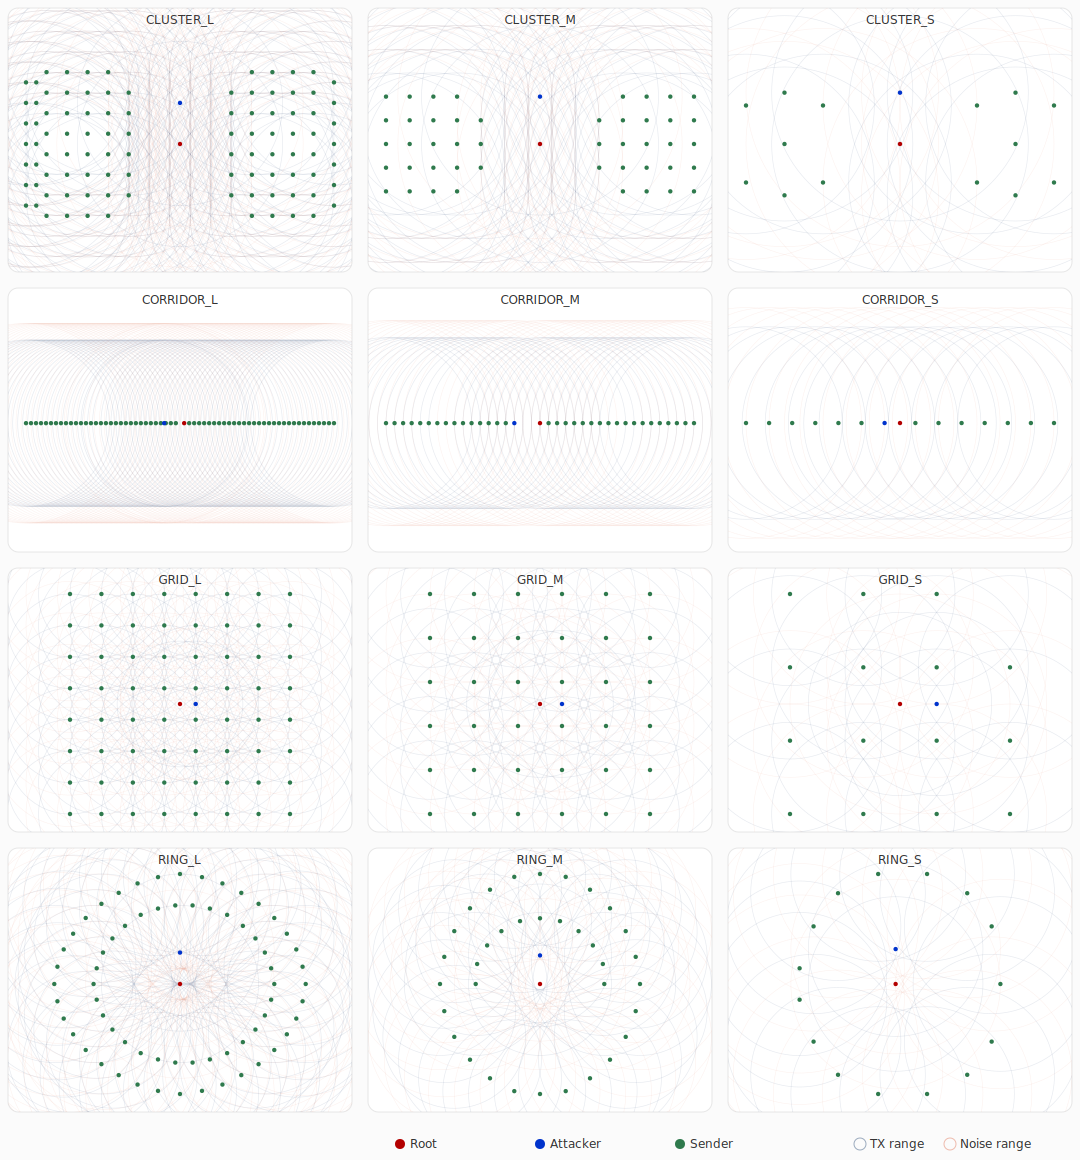
\includegraphics[width=\textwidth,height=\textheight,keepaspectratio]{topology_svgs/all_topologies.pdf}
  \caption{Topology layouts used for evaluation, covering different path diversity regimes and attacker positions.}
  \label{fig:all-topologies}
\end{figure}

\subsection{Attack Configuration}
Selective forwarding은 drop probability(예: 0/30/50/70\%)로 parameterize한다. Sinkhole intensity는 rank manipulation delta(예: 1/2/4)로 parameterize한다. 세 가지 mode를 평가한다: selective forwarding only, sinkhole only, combined.

\begin{figure}[t]
  \centering
  \includegraphics[width=0.9\linewidth]{experiment_workflow.pdf}
  \caption{Experiment workflow from simulation execution to offline metric extraction.}
  \label{fig:workflow}
\end{figure}

\subsection{Trust Model Parameters}
\label{subsec:trust-params}
Table~\ref{tab:trust-params}는 실험 전반에서 사용한 trust 관련 parameter를 요약한다. 별도로 명시하지 않는 한, scenario별 튜닝을 피하기 위해 모든 topology 및 scale에 동일 구성을 적용한다.

\begin{table}[t]
\centering
\caption{Trust model parameters used in experiments.}
\label{tab:trust-params}
\begin{tabular}{lll}
\toprule
Parameter & Description & Value \\
\midrule
$\alpha_0$ & Beta prior (success) & 1 \\
$\beta_0$  & Beta prior (failure) & 1 \\
$\rho$     & EWMA smoothing factor & 0.8 \\
$W$        & Rank stability window & 5 sampling intervals \\
$\tau$     & Rank deviation tolerance & 0 \\
$\kappa$   & Rank increase tolerance & 0 \\
$\lambda_{\text{adv}}$ & Rank anomaly sensitivity & 0.01 \\
$\lambda_{\text{stab}}$ & Rank instability sensitivity & 0.01 \\
$w_1$      & Weight of rank inconsistency trust & 0.5 \\
$w_2$      & Weight of rank stability trust & 0.5 \\
$\alpha$   & Grayhole vs. sinkhole trust weight & \{1.0, 0.5\} \\
$\lambda$  & Trust penalty strength & \{0, 1, 3, 10\} \\
$\gamma$   & Risk sensitivity exponent & \{1, 2, 4\} \\
\bottomrule
\end{tabular}
\end{table}

\subsection{Metrics}
다음 metric을 보고한다:
\begin{itemize}[leftmargin=*]
  \item \textbf{PDR:} $\mathrm{RX}_{\text{root}} / \mathrm{TX}_{\text{senders}}$.
  \item \textbf{End-to-end delay:} source에서 root까지의 per-packet latency.
  \item \textbf{Control overhead:} control-plane transmission(예: DIO/DAO) 및 routing-related overhead.
  \item \textbf{Parent churn:} parent switching rate로, routing stability를 반영.
  \item \textbf{Exposure (optional):} delivered packet 중 attacker를 traverse한 비율 및/또는 attacker가 preferred parent인 시간 비율(attack effectiveness 해석용).
\end{itemize}

\subsection{Parameter Sweeps}
다음을 스윕한다:
(i) attack intensity,
(ii) topology class 및 scale,
(iii) trust aggregation weight $\alpha$,
(iv) trust-aware case에 대한 penalty parameter $(\lambda,\gamma)$.
Mean 및 variability를 보고하기 위해 multiple random seed를 사용한다.

\begin{table}[t]
\centering
\caption{Core experimental parameters (default).}
\label{tab:params}
\begin{tabular}{ll}
\toprule
Parameter & Value \\
\midrule
Field size & 200 m $\times$ 200 m \\
Radio model & UDGM Distance Loss \\
TX range / Interference range & 45 m / 90 m \\
Simulation time / Warm-up & 600 s / 120 s \\
Traffic interval & 30 s \\
Root ID & 1 \\
Attacker count & 1 (default) \\
\bottomrule
\end{tabular}
\end{table}

\section{Results}
\label{sec:results}
본 절은 데이터 수집 이후 최종화한다. 분석은 (i) collapse threshold behavior와 (ii) trust penalization으로 유발되는 trade-off를 강조하도록 구성한다.

\begin{figure}[t]
  \centering
  \fbox{\parbox{0.9\linewidth}{\centering Fig.~3 (placeholder): PDR vs. attack intensity by topology/scale}}
  \caption{PDR vs. attack intensity (placeholder).}
  \label{fig:pdr}
\end{figure}

\begin{figure}[t]
  \centering
  \fbox{\parbox{0.9\linewidth}{\centering Fig.~4 (placeholder): delay vs. attack intensity}}
  \caption{End-to-end delay vs. attack intensity (placeholder).}
  \label{fig:delay}
\end{figure}

\begin{figure}[t]
  \centering
  \fbox{\parbox{0.9\linewidth}{\centering Fig.~5 (placeholder): control overhead vs. attack intensity}}
  \caption{Control overhead vs. attack intensity (placeholder).}
  \label{fig:overhead}
\end{figure}

\begin{figure}[t]
  \centering
  \fbox{\parbox{0.9\linewidth}{\centering Fig.~6 (placeholder): parent churn vs. attack intensity}}
  \caption{Parent churn vs. attack intensity (placeholder).}
  \label{fig:parent-switch}
\end{figure}

\begin{figure}[t]
  \centering
  \fbox{\parbox{0.9\linewidth}{\centering Fig.~7 (placeholder): $(\lambda,\gamma)$ sweep trade-off surface}}
  \caption{Trade-off under trust penalty sweeps (placeholder).}
  \label{fig:lambda-tradeoff}
\end{figure}

\section{Discussion}
\label{sec:discussion}
Topology-dependent path diversity와 attacker placement가 collapse threshold에 미치는 영향, 그리고 trust penalization이 threshold를 어떻게 이동시키는지 논의한다. 또한 (i) wireless loss 및 transient dynamics에서의 false positive 가능성, (ii) $(\lambda,\gamma,\alpha)$에 대한 sensitivity, (iii) churn 및 overhead에 반영되는 stability 영향을 분석한다. 제안 메커니즘은 cryptographic protection 및 secure bootstrapping을 \emph{대체}하는 것이 아니라 \emph{보완}하기 위한 것으로, full authentication이 불가능하거나 비실용적인 환경에서도 resilience gain을 제공하는 것을 목표로 한다.

\section{Conclusion and Future Work}
\label{sec:conclusion}
본 논문은 data-plane reliability 및 control-plane anomaly signal을 함께 활용하여 BRPL routing decision에 경량 trust penalty를 통합한 Trust-Aware BRPL을 제시하였다. 평가 설계는 selective forwarding 및 sinkhole attack 하에서 trust parameter가 performance collapse를 얼마나 지연시키는지 정량화하고, topology 및 scale 전반에서 resilience--overhead trade-off를 특성화하도록 구성된다. 향후 연구로는 colluding multiple attacker, trust penalty parameter의 adaptive tuning, real testbed에서의 validation을 포함한다.

\bibliographystyle{plainnat}
\bibliography{references}

\end{document}
